\chapter{LAPORAN}
\section{TUGAS TEORI}
\begin{itemize}
\item Pengertian, sejarah, fungsi dan contoh file csv
\begin{enumerate}
    \item Pengertian\\
    CSV merupakan singkatan dari Comma Separated Values, merupakan suatu format file/data yang setiap recordnya dipisahkan dengan menggunakan koma (,) atau dapat juga menggunakan titik koma (;) sebagai pemisah di antara elemen yang ada. Format file csv dapat dibuka melalui text editor yang biasa dijumpai, contohnya notepad, excel, wordpad.
    \item Sejarah
    nilai data ynag dipisahkan dengan menggunakan tanda koma ialah format data yang memberi tanggal lebih awal pada personal computer
    Nama dan singkatan yaitu csv digunakan pada 1983 secara manual untuk komputer Osborne Executive yang menggabungkan SuperCalc spreadsheet, mendokumentasikan konvemsi kutipan csv yang memungkinkan text/string berisi koma. Data yang dipisahkan dengan tanda baca koma lebih mudah untuk diketik.\\
    Pada tahun 2014 IETF menerbitkan RFC7111 yang menjelaskan tentang aplikasi fragmen URI ke dokumen csv. RCF7111 menentukan rentang baris, kolom, dan sel yang dapat dipilih dari dokumen csv menggunakan indeks posisi. Kemudian pada tahun 2015 menerbitkan W3C dalam upaya untuk meningkatkan csv dengan semantik formal, mempublikasikan draft rekomendasi pertama sebagai standard metadata csv yang dimulai sebagai rekomendasi yang ada pada bulan Desember tahun 2015.
    \item Fungsi\\
    untuk memudahkan dalam memindahkan data dari suatu program ke program yang lainnya.
    \item Contoh
     npm,namalengkap, kelas\\
     1184030,Dyning Aida ,D4TI2B\\
     1184051,Alifia Zahra ,D4TI2B\\ 
\end{enumerate}
\item Aplikasi yang dapat menciptakan file csv\\
\begin{enumerate}
    \item Text Editor, contohnya Notepad, wordpad
    \item Speadsheet berupa Microsoft Excel
\end{enumerate}
\item Cara menulis atau membaca file csv di excel atau spreadsheet
\begin{enumerate}
    \item Buatlah dokumen baru di microsoft excel
    \item Tambahkan judul kolom untuk setiap informasi yang ingin dicatat, contohnya npm, namalengkap, dan kelas. Lalu ketikkan isi dari kolom tersebut dengan sesuai. Setelah itu data yang dibuat di excel akan terlihat seperti gambar berikut :\\
    \item Simpan file dalam format csv
\end{enumerate}
\item Sejarah library csv\\
Format csv ialah format yang digunakan selama bertahun-tahun sebelum adanya upaya untuk menggambarkan format standar pada RFC 4180.
\item Sejarah library pandas\\
Pandas ialah toolkit yang powerful untuk digunakan sebagau alat untuk menganalisis data dan struktur pada bahasa pemrograman Python. Salah satu fitur yang ada pada pandas ialah Dataframe yang digunakan untuk mengolah data dengan mudah.
\item Fungsi-fungsi yang terdapat di library csv\\
Berikut ini fungsi -fungsi yang terdapay di library csv, di antaranya yaitu
\begin{enumerate}
\item reader\\
Reader merupakan fungsi yang digunakan untuk membaca isi file csv dari list. Berikut ini merupakan contoh penggunaannya
\lstinputlisting[language=Python]{src/open.py}
\item write\\
Write merupakan fungsi yang digunakan untuk menulis file csv dari list. Berikut ini merupakan contoh penggunaannya
\lstinputlisting[language=Python]{src/write.py}
\item DictRead\\
Merupakan fungsi yang digunakan untuk membaca isi file csv dari dictionary. Berikut ini merupakan contoh penggunaannya
\lstinputlisting[language=Python]{src/dictread.py}
\item DictWrite\\
Merupakan fungsi yang digunakan untuk menulis isi file csv dari dictionary. Berikut ini merupakan contoh penggunaannya
\lstinputlisting[language=Python]{src/dictwrite.py}
\end{enumerate}
\item Fungsi-fungsi yang terdapat di library pandas\\
Berikut ini merpakan fungsi dari library pandas, di antaranya yaitu :
\begin{enumerate}
    \item read csv\\
    Read csv merupakan fungsi yang digunakan untuk membaca file csv dengan library pandas
    \lstinputlisting[language=Python]{src/readcsvp.py} membaca file csv dengan pandas
    \item to csv\\
    Merupakan fungsi yang digunakan untuk menulis file csv menggunakan library pandas
    \lstinputlisting[language=Python]{src/tocsv.py} menulis file csv dengan fungsi to csv
\end{enumerate}
\end{itemize}
\section{KETERAMPILAN}
1. Open file dengan Mode List
\lstinputlisting[language=Python]{src/open.py} 
2. Open file dengan Mode Dictionary
\lstinputlisting[language=Python]{src/dictwrite.py}
3. Open file csv dengan lib pandas mode list
\lstinputlisting[language=Python]{src/1184030pandas.py}
4. Open file csv dengan lib pandas mode dict 
\lstinputlisting[language=Python]{src/1184030pandas2.py}
5. \lstinputlisting[language=Python]{src/1184030pandas3.py}
6. \lstinputlisting[language=Python]{src/1184030pandas4.py}
7. \lstinputlisting[language=Python]{src/1184030pandas5.py}
8. \lstinputlisting[language=Python]{src/main.py}
9. \lstinputlisting[language=Python]{src/main2.py}
\section{KETERAMPILAN PENANGANAN ERROR}
\begin{enumerate}
\item peringatan error pada praktek ketiga dan penjelasan penanganan error tersebut.\\
Peringatan error yang muncul salah satunya yaitu seperti gambar di bawah ini :\\
\lstinputlisting[language=Python]{src/2err.py}
		Cara penanganan yang digunakan untuk mengatasi error tersebut yaitu dengan memberikan try untuk menghasilkan/mencetak fungsi sebelumnya, kemudian jika parameter yang ditangkap tidak sesuai maka, program akan mengeksekusi exception dan mencetak peringatannya.
\end{enumerate}
\section{SCAN PLAGIARISME}
                \begin{figure}[H]
				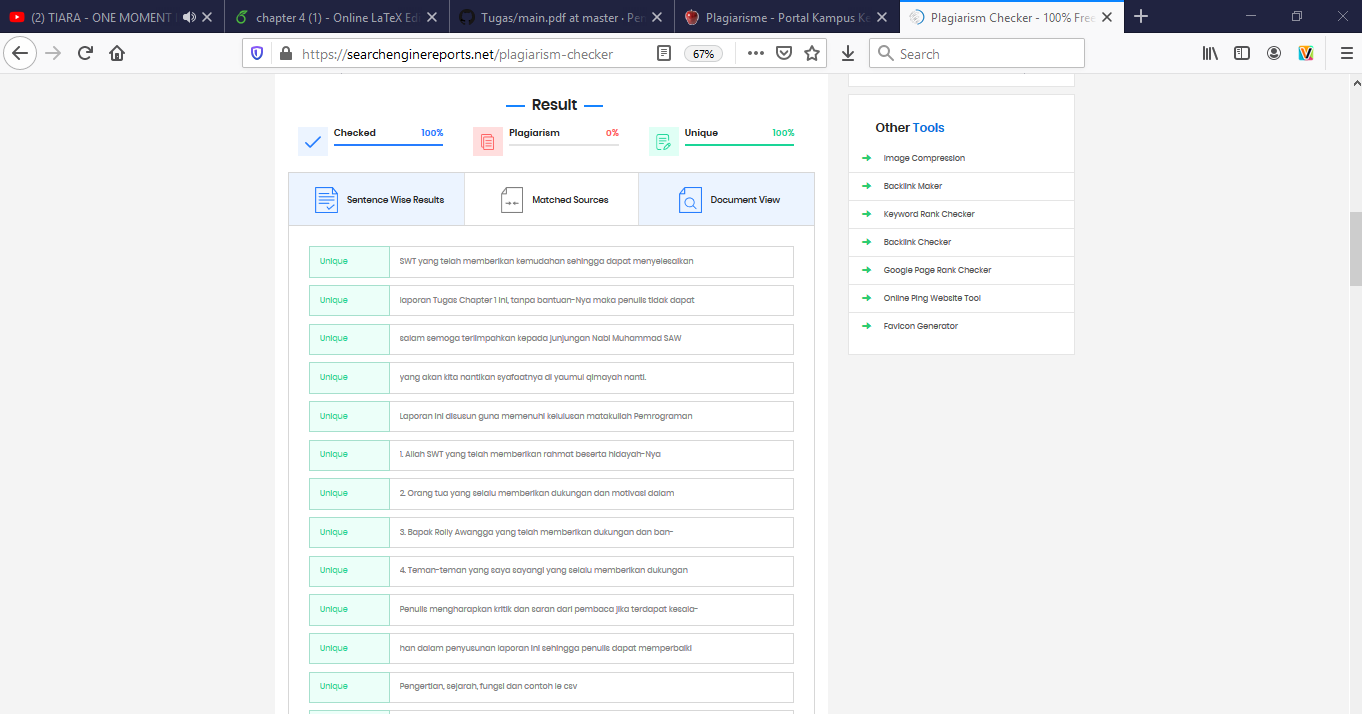
\includegraphics[width=20cm]{figures/plagiarisme.PNG}
				\centering
				\caption{hasil scan plagiarisme}
				\end{figure}